\section{Preliminary Results}
\label{sec-results}

To collect spectrum utilization information, Wifi cards needs to be put in
monitor mode so that every decoded packet is delivered to upper layer.  However,
almost none of current smartphone hardwares support monitor mode, at
least without firmware and driver hacking~\cite{bcmon}. To mitigate this
limitation, we use external Wifi dongle to mimic future smartphone hardwares
with built-in monitor mode support. Table~\ref{tab:dongle} shows the
specification of the Wifi dongle used in our experiments. The dongle is
connected to smartphone (Galaxy Nexus) through OTG cable. We refer a smartphone
with Wifi dongle as \textit{sniffer device} hereafter.

\begin{table}[t!]
  \centering
  \begin{tabular}{ll}
    \toprule
    \textbf{Model} & ALFA Network AWUS036H \\
    \textbf{Chipset} & RTL8187L \\
    \textbf{Connector} & $1\times2.4$GHz SMA \\
    \textbf{Antenna} & 2.5dBi rubber duck \\
    \textbf{Wifi Support} & 802.11b/g \\
    \bottomrule
  \end{tabular}
  \caption{Wifi dongle specification.}
  \label{tab:dongle}
\end{table}


\subsection{Rogue Access Point}

Rogue Access Point (RAP) are unauthorized APs that connected to secure corporate
network. They pose security vulnerabilities as well as undesired Radio Frequency
(RF) interferences to usually well planed corporate networks. Most RAPs are set
up by employees for their own convenience. Thus besides being able to simply
detect the existence of RAPs, it's also interesting to see their impacts: how
many devices the RAP serve and how much traffic it generates. Intuitively, RAPs 
that serve many devices may imply certain \textit{coverage holes} of the
corporate network. And the traffic volume generated by RAPs should be a hint to
the network administrator when evaluating their RF interference.

In this experiment, we deploy 6 sniffer devices to investigate the RAPs in our
department building.  3 of them are deployed statically in public areas such as
laboratory, corridor and lounge. And others are carried by the authors on daily
basis. The devices are put in monitor mode to keep sniffing packets in the air.
In total, 38 device-hour's data (contains 37M packets) are captured.  

We first inspect beacon frames to identify APs. Then we exclude campus APs and
temporary hotspots with less than 1000 beacon frames. 56 RAPs were
detected in this way. For each RAP, we calculate the traffic volume (both
down and up link) by summing up the length of all data frames.
Figure~\ref{fig:rap} shows 15 RAPs with most traffic, as well as the number of
devices that ever exchange data frames with them.

\begin{figure}[t!]
  \centering
  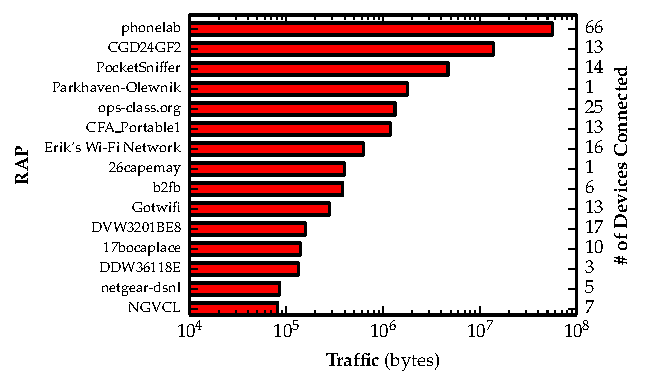
\includegraphics[width=0.48\textwidth]{./figures/RAPTrafficGraph.pdf}
  \caption{Rogue AP traffic detected by sniffer device.}
  \label{fig:rap}
\end{figure}

Among these 15 RAPs, \texttt{phonelab} and \texttt{ops-class.org} are known to
be open access APs set up by the authors.  They both generate a large amount of
traffic and serve a fair large number of devices, which indicates potential
coverage holes of the campus network. Other RAPs, such as
\texttt{Parkhaven-Olewnik} and \texttt{26capemay}, also generated large traffic
volume yet all of them are with one device. This indicates typical personal RAPs
that are secured and only used by the owner.


\subsection{Channel Assignment}

To demonstrate the feasibility of using client-side measurements to improve
channel assignment, we built an concept-proof system, where a sniffer device,
when connected to \PS{}-enabled APs, will periodically collect
and report the traffic condition on all channels. The AP, which runs a tiny 
server on top of custom firmware, periodically selects the least congested
channel base on all associated client's measurements.

The experiment is designed as follows. We first set up a constant \texttt{iperf}
UDP traffic at 15 Mbps between \PS{}-AP $A$ and sniffer device $D_1$ on channel
$C_1$. Then another device, $D_2$, starts jamming the channel by sending
saturated UDP traffic. Since $D_1$ periodically collects and reports traffic
information, $A$ will eventually realize this interference from $D_2$ and find
another less congested channel $C_2$ and switch to it. All devices in this
experiment are using 802.11g at 2.4GHz band. 

In the particular run showed in Figure~\ref{fig:bw}, from 0s to 8.5s, $A$ and
$D_1$ establish stable UDP traffic on channel 11. Then $D_2$ starts jamming the
channel, the link bandwidth between $A$ and $D_1$ decreased and fluctuated due
to the interference. At 75s, when $A$ and $D_1$ switch to a less congested
channel (1), the bandwidth resumes to previous level before the interference.

\begin{figure}[t!]
  \centering
  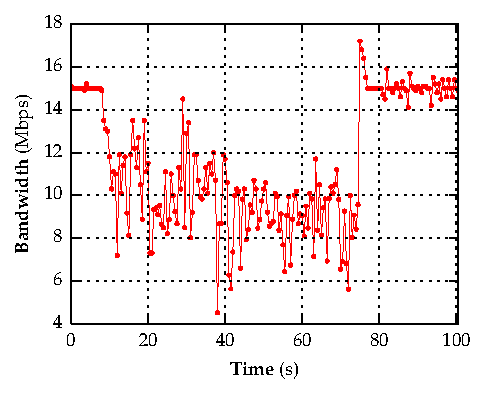
\includegraphics[width=0.48\textwidth]{./figures/ChannelBWGraph.pdf}
  \caption{Instaneous bandwidth between $A$ and $B_1$ after jamming (8.5s) and
  channel switching (75s).}
  \label{fig:bw}
\end{figure}
